{ The objective addressed in this Section is to develop a procedure to
  identify spectral bands that yield good temperature, gravity and
  metallicity diagnostics. Given the lack of a calibration set of
  observed spectra with homogeneous coverage of the space of physical
  parameters, we turn to synthetic libraries of spectra. The atomic or
  molecular line/band parameters could in principle indicate the
  spectral features that are more sensitive to changes in the physical
  parameters. The suitability of spectral features as diagnostics
  ofthe stellar atmospheric properties depends not only on the
  individual behaviour of each line/band, but also on the relative
  properties of neighbouring features in the same spectral region,
  that may overlap depending on the spectral resolution. Furthermore,
  good spectral diagnostics at a given signal-to-noise ratio (SNR) may
  show a severy degraded predictive power in the low SNR regime. In
  the following we adopt the BT-Settl library of synthetic spectra
  (\cite{2013MSAIS..24..128A}) as the framework where spectral
  diagnostics will be searched for. These synthetic spectra were
  pre-processed in several steps as described below.}

{ First, and in order to define good temperature diagnostics, spectra
between 2000 and 4200K in steps of 100 K were selected, with $\log(g)$
in the range between 4 and 6 dex (when g is expressed in cm/s$^{-2}$),
in steps of 0.5 dex. The metallicity of the representative spectra was
restricted to the set 0, 0.5 and -1 dex.  This yields a total set
size of 535 available spectra.

{A series of preprocessing steps were then carried out in order to
match the spectral resolution and wavelength coverage and sampling of
the synthetic library to that of the collection of observed spectra
(IPAC or IRTF, see below). This required the definition of a common
wavelength range present in all available observed spectra, and the
subsequent trimming to match that range. A unique wavelength sampling
was also defined and all spectra (synthetic and observed) interpolated
to match the sampling. Finally, all spectra, both synthetic and
observed were divided by the integrated flux in order to factor out
the stellar distance.}

{ In order to increase the density of examples in parameter space, we
  introduced interpolated spectra in the BT-Settl grid. Interpolation
  was obtained as a linear combination of spectra in the grid,
  weighted by the inverse square of the euclidean distance. {\bf Aqui,
  la distancia euclidea deberia calcularse en parametros normalizados,
  porque si no la temperatura domina la distancia. Fue asi?} We
  compared a set of interpolated spectra with those produced using the
  PHOENIX code (\cite{fuhrmeister2005phoenix}) to be sure that
  interpolation was a valid solution to infer new synthetic
  spectra. {\bf Yo aqui daría el RMSE de reconstruccion, mejor que la
  figura comp-gen-inter}

%(see Fig.~\ref{fig:comp_gen_inter}).  }

%\begin {figure}
% \begin{center}
% 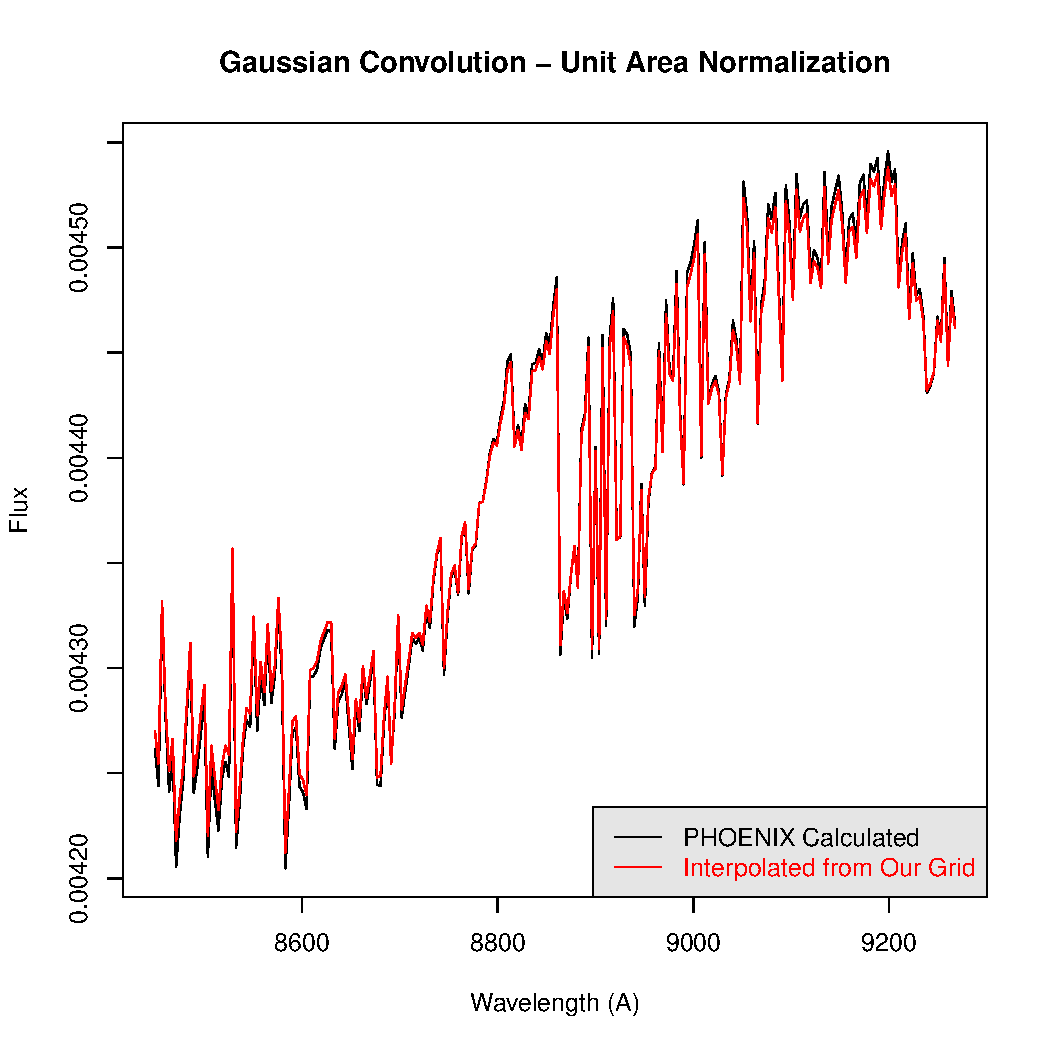
\includegraphics[width=6cm]{figs/intgrid4_gauss.pdf}
% \caption{Comparison between generated and interpollated spectrum}
% \label{fig:comp_gen_inter}
% \end{center}
%\end {figure}

{ A first interpolation stage allowed us to define a finer mesh step of
0.25 dex for both, $\log(g)$ and metallicity and 50K in temperature,
yielding a total 1329 spectra.  Then, a second interpolation stage
refined the grid down to 25 K in temperature and 0.125 dex in 
$\log(g)$, keeping the metallicity step at 0.25 dex and producing a
dataset with 25912 spectra.}

{In spite of these, and in order to keep their knowledge closer to the
original BT-Settl source, most of the analyses have been performed
with the original 535 spectra dataset.  }{\bf Habría que delimitar
exactamente donde se han utilizado 535 y dónde 25912. Si la mayoria
del analisis se ha realizado sobre 535, no se si tiene sentido incluir
la parte de interpolacion.}


{ In order to avoid selecting spectral features that are good
  predictors only in the unrealistic SNR=$\infty$ regime, the search
  for optimal diagnostics of the atmopheric paramters of M stars was
  carried out for three SNR values (10, 50 and $\infty$) by degrading
  the synthetic spectra with Gaussian noise of zero mean.  {\bf Quizás
  deberíamos citar el trabajo de Ana como in preparation} }

\subsection{Feature definition and selection}
\label{subsec:FD}
{ As mentioned in Sect. \ref{sec:intro}, it is well known the
difficulty in defining good spectral diagnostics for M stars in the
infrared.}

{The work in \cite{2013A&A...549A.129C} defined wavelength regions in
the I and K bands optimal for the diagnostic of physical parameters
based on the sensitivity exhibited by the flux emitted in these
segments to changes of the physical parameters. The sensitivity was
measured in terms of the derivative of the flux with respect to the
physical parameter. The approach adopted in this work is to select
spectral features that yield the best accuracy when used as predictive
variables in a regression model that estimates the stellar atmospheric
physical parameters ($T_{eff}$, $\log(g)$ and metallicity). The
evaluation of the accuracy of the estimates produced from a subset of
features is described further below. We consider the effective
temperature as the dominant parameter influencing changes in the
stellar spectra (a strong feature) and thus, it was estimated first,
and then used as in the regression models for the gravity and
metalicity.}

Here, a feature $F$ is defined as

\begin{equation}\label{eq:feature}
  F = \int_{\lambda_{1}}^{\lambda_{2}} (1-\frac{f(\lambda)}{F_{cont}} \cdot {\rm d}{\lambda})
\end{equation}

where $f(\lambda)$ denotes the normalized flux from the star at
wavelength $\lambda$, and where $F_{cont}$ is the average flux in a
spectral band between $\lambda_{cont;1}$ and $\lambda_{cont;2}$. We
explain below how we search for the band definitions that produce
physical parameter predictions with the smallest errors.

{\bf Aquí he omitido los detalles sobre las restricciones a las bandas
porque no lo entiendo bien. ¿Podrías explicarlo con palabras en lugar
de items?}

%\begin{itemize} \item { $ \vert \lambda_{2k(i)}
% - \lambda_{1k(i)} \vert = 30 $ pixels of spectrum $ \quad \forall
% i \in [1 \ldots N]$ and $ k \in \{s,c\} $ .}  \item { $ min
% ( \lambda_{1k(i)}, \lambda_{1k(j)} ) = 5 $ pixels of spectrum
% $ \quad \forall i,j \in [1 \ldots N] $ ; $ i \neq j $ and $
% k \in \{s,c\} $ .}  \item {
% $ \overline{\lambda_{2}(i)\lambda_{1}(i)} \bigcap \overline{\lambda_{2c}(i)\lambda_{1c}(i)}
% = \emptyset \quad \forall i \in [1 \ldots N]$.}  \end{itemize}
%which become a guarantee avoiding any overlap 
%and a minimum size for both signal and continuum bandpasses.

Another type of features defined as

\begin{equation}\label{eq:feature2}
  F' = \frac{ \int_{\lambda_{1}}^{\lambda_{2}}f(\lambda) \cdot {\rm d}{\lambda}}
               {\int_{\lambda_{3}}^{\lambda_{4}} f(\lambda) \cdot {\rm d}{\lambda}} 
\end{equation}

was considered, where $\lambda_1, \lambda_2, \lambda_3$, and
$lambda_4$ delimit two spectral bands such that the ratio of the
integrated fluxes in the two bands is hoped to be a good predictor
(alone or in combination with other features) of the star atmospheric
physical parameters. The results obtained with this alternative
feature definition did not differ significantly on average from the
ones observed with the one adopted in Eq. \ref{eq:feature}, and
including them here would result in an excessively lengthy paper. In
view of the equivalent global performances, we prefered the former
because it allows direct comparison with the features proposed
by \cite{2013A&A...549A.129C}.

We used Genetic Algorithms to solve the optimization problem described
above, that is, the problem of finding the features (band boundaries)
that minimize the prediction error of a regression estimate of the
physical parameters. We used the implementation of genetic algorithms
publicly available as the R \citep{R2013} ???  package.

%These methods have demonstrated to perform well ({\bf falta cita})
%{\bf ¿en qué circunstancias?}. However, in some cases they can be
%ineffective regardless of the classification method used. An obvious
%conceptual limitation of univariate approaches is also the lack of
%consideration that features works in the contexts of interconnected
%pathways and therefore it is their behavior as a group that may be
%predictive of the phenotypic variables. Multivariate selection methods
%%may seem to be more suitable for the analysis of data since variables
%are tested in combination to identify interactions between
%features. However, the extremely large number of models that can be
%constructed from different combination of thousands of features cannot
%be extensively evaluated using standard computational resources.

For the sake of simplicity let us define Genetic Algorithms (GAs) as
search algorithms that are based on the principle of evolution by
natural selection. The procedure works by evolving (in the sense
explained below) sets of variables (chromosomes) from an initial
random population. Evolution proceeds via cycles of differential
replication, recombination and mutation of the fittest
chromosomes. The concept of fittest is context dependent, but in our
case fitness is defined in relation with the accuracy with which a
given chromosome (set of spectral features ${F_i}$) predicts the
physical parameters. The concept of using in-silico evolution for the
solution of optimization problems was introduced
by \cite{holland1975adaptation}. Although its application is now
reasonably widespread \citep[see e.g. ]{goldberg1989genetic}), they
became very popular only when sufficiently powerful computers became
available. {\bf Aquí hay que citar trabajos en astrofísica que
utilicen GA y, en particular, un artículo de Charbonneau
http://adsabs.harvard.edu/abs/1995ApJS..101..309C en 1995 que fue como
la presentación en sociedad.}

The implementation of the GA comprises the following steps:

\begin{itemize}
\item [\textbf{Stage 1}:]{Definition of the population of potential features (chromosomes).}
\item [\textbf{Stage 2}:]{Each chromosome in the population is evaluated by its ability to
predict the physical paramters of each star in the dataset (fitness
function).}
\item [\textbf{Stage 3}:]{Chromosome selection, when a chromosome has 
 a score higher then a predefined value.}
\item [\textbf{Stage 4}:]{The population of chromosomes is replicated. 
 Chromosomes with a higher fitness score will generate a more numerous
 offspring.}
\item [\textbf{Stage 5}:]{The genetic information contained in the replicated parent
chromosomes is combined through genetic crossover. Two randomly
selected parent chromosomes are used to create two new chromosomes.}
\item [\textbf{Stage 6}:]{Mutations are then introduced in the chromosome randomly. 
 These mutations produce new genes used in chromosomes.  Steps 5 and 6
 are applied over the chromosomes established at Step 4.}
\item [\textbf{Stage 7}:]{This process is repeated from Stage 2 until 
  a target accuracy is achieved or the maximum number of iterations is
  attained.}
\end{itemize}

{\bf Es muy importante definir la codificación del cromosoma. ¿Es la
codificación de un único feature? ¿un subconjunto de features? ¿de qué
tamaño?}

There are different statistics that can be used to identify features
that are differentially expressed between two or more groups of
samples {\bf hay que explicar a qué nos referimos con differential
expression, samples y groups of samples aquí} and then uses the most
differentially expressed to construct a statistical model.

The population size was set to 1000 individuals and the maximum number
of accepted iterations set to 4000. We produced three randomly started
populations so as to provide enough initial variety. The crossover and
mutation probabilities were set to 0.85 and 0.35 respectively. Elitism
was fixed to 0.15 {\bf No hemos mencionado elitismo; hay que
mencionarlo y definirlo antes}.  Feature fitness was defined in terms
of the Akaike Information Criterion (AIC) for linearity between the
potential feature against the physical parameter. {\bf No entiendo
esta última frase. La linealidad... ¿se refiere al modelo de regresión
lineal que utilizamos para medir el fitness de una feature? Creo que
hay que añadir un párrafo en el que expliquemos con detalle el
regresor utilizado para medir la fitness. Y sobre todo, aclarar si el
cromosoma codifica sólo una feature o un conjunto de features.} The
most frequent and efficient features were selected as candidates to
predictive variables of the physical parameters in regression
models. We used a binary codification of the chromosomes and a
parallel implementation of the GA in a farm of fifteen computers per
physical parameter.

The GA procedure provides us with a large collection of chromosomes.
Although these are all potential solutions of the problem, it is not
immediately clear which one should be selected for the final
regression model.  This single regression model should, to some
extent, be representative of the population. The simpler strategy
would be to use the frequency of the chromosome in the population as
criterion for inclusion in a forward selection strategy. However we
prefered to select the features based on their highest fitness.
  
